\documentclass[
11pt, % Set the default font size, options include: 8pt, 9pt, 10pt, 11pt, 12pt, 14pt, 17pt, 20pt
%
aspectratio=169, % Uncomment to set the aspect ratio to a 16:9 ratio which matches the aspect ratio of 1080p and 4K screens and projectors
]{beamer}

\graphicspath{{Images/}{./}} % Specifies where to look for included images (trailing slash required)
\usepackage{booktabs} % Allows the use of \toprule, \midrule and \bottomrule for better rules in tables

%\usepackage{appendixnumberbeamer} %If you want a separate slide counter for your appendix

%%% Customize Theme %%%%%%%%%%%%%%%%%%%%%%
\usetheme{Madrid} % You can use other themes too, but this changes many things. I've found Madrid to be the best for this color scheme

%fg = font color
%bg = background color

% ! WARNING ! : Many colors are linked to multiple attributes, so changing one color can have unexpected changes!

% If you want to tweak the shading of orange and red, tweak the below 2 lines:t
\definecolor{myGreen}{RGB}{1, 1, 122}
\definecolor{myDarkGreen}{RGB}{1, 1, 122}

% Bottom right hand color
\setbeamercolor*{structure}{bg=myGreen!20,fg=myGreen!90}

\setbeamercolor*{palette primary}{use=structure,fg=white,bg=structure.fg} %?
\setbeamercolor*{palette secondary}{use=structure,fg=myGreen,bg=white}
%bottom left of footer & bar between title & top bubbles
\setbeamercolor*{palette tertiary}{use=structure,fg=white,bg=myGreen} 

\setbeamercolor{frametitle}{bg=myGreen!85,fg=white} %title of each slide

\setbeamercolor*{titlelike}{parent=palette primary} %?
%\setbeamercolor{titlelike}{parent=palette primary,fg=structure.fg!50!myRed}

%for miniframe (very top) AND center footer
\setbeamercolor{section in head/foot}{fg=myDarkGreen, bg=white}

%%% Specific Colors %%%
\setbeamercolor{item projected}{bg=myDarkGreen}
\setbeamertemplate{enumerate items}{bg=myOrange}

\setbeamercolor{itemize item}{fg=myDarkGreen}
\setbeamercolor{itemize subitem}{fg=myDarkGreen}

\setbeamercolor{button}{bg=myDarkGreen}

%%% Edits ONLY the TOC slide %%%
\setbeamercolor{section in toc}{fg=black}
\setbeamercolor{subsection in toc}{fg=black}

%%% Block Colors %%%
% Standard block %
\setbeamercolor{block title}{bg=myDarkGreen, fg=white}
\setbeamercolor{block body}{bg=myDarkGreen!20}

% Alerted block % If you want to customize it's color
%\setbeamercolor{block title alerted}{bg=cyan, fg=white}
%\setbeamercolor{block body alerted}{bg=cyan!10}

% Example block % If you want to customize it's color
%\setbeamercolor{block title example}{bg=cyan, fg=white}
%\setbeamercolor{block body example}{bg=cyan!10}

%---------------------------------------------------------
%	SELECT FONT THEME & FONTS
%---------------------------------------------------------
\usefonttheme{default} % Typeset using the default sans serif font
\usepackage{palatino} % Use the Palatino font for serif text
\usepackage[default]{opensans} % Use the Open Sans font for sans serif text
\useinnertheme{circles}

%---------------------------------------------------------
%	SELECT OUTER THEME
%---------------------------------------------------------
% Outer themes change the overall layout of slides, such as: header and footer lines, sidebars and slide titles. Uncomment each theme in turn to see what changes it makes to your presentation.

%\useoutertheme{default}
%
\useoutertheme{miniframes}

%\useoutertheme{infolines}
%\useoutertheme{smoothbars}
%\useoutertheme{sidebar}
%\useoutertheme{split}
%\useoutertheme{shadow}
%\useoutertheme{tree}
%\useoutertheme{smoothtree}

%---------------------------------------------------------
%	PRESENTATION INFORMATION
%---------------------------------------------------------

\title[]{Modelación de la Especialización Hemisférica del Cerebro para Frecuencias Espaciales a través de Campos Receptivos Poblacionales}
\subtitle{}
\author[Mari\'e del Valle Reyes]{Mari\'e del Valle Reyes}

\institute[]{\textbf{Tutores:} \\ Dr. Mitchell Valdes Sosa\\ Msc. Ania Mesa Rodr\'iguez }

\date[enero de 2024]

%\date[\today]



%---------------------------------------------------------
%---------------------------------------------------------
%---------------------------------------------------------
\begin{document}
	
	%---------------------------------------------------------
	%	TITLE SLIDE
	%---------------------------------------------------------
	\section{}
	\begin{frame}
		\titlepage % Output the title slide, automatically created using the text entered in the PRESENTATION INFORMATION block above
		
	\end{frame}
	
	%---------------------------------------------------------
	%	TABLE OF CONTENTS SLIDE
	%---------------------------------------------------------
	% The table of contents outputs the sections and subsections that appear in your presentation, specified with the standard \section and \subsection commands. You may either display all sections and subsections on one slide with \tableofcontents, or display each section at a time on subsequent slides with \tableofcontents[pausesections]. The latter is useful if you want to step through each section and mention what you will discuss.
	
	\begin{frame}
		\frametitle{Contenidos} % Slide title, remove this command for no title
		
		\tableofcontents % Output the table of contents (all sections on one slide)
		%\tableofcontents[pausesections] % Output the table of contents (break sections up across separate slides)
	\end{frame}
	
	%---------------------------------------------------------
	%	PRESENTATION BODY SLIDES
	%---------------------------------------------------------


     \section{El Cerebro}
     
      \begin{frame}
     	\frametitle{El Cerebro}
     	
     	\begin{columns}[c] % The "c" option specifies centered vertical alignment while the "t" option is used for top vertical alignment
     		\begin{column}{0.3\textwidth} % Right column width
     			\centering
     		Sistema complejo\\
     		que regula y controla la mayor\'ia
     		de las funciones del cuerpo y la mente.
     			
     			
     		\end{column}
     		
     		\begin{column}{0.3\textwidth}
       		\begin{figure}
     			\centering
     			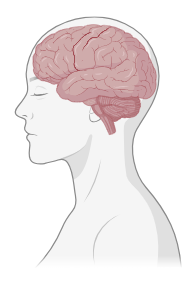
\includegraphics[scale=0.7]{Graphics/female_brain}
     		\end{figure}
     		\end{column}
     		
     		\begin{column}{0.3\textwidth} % Left column width
     			\centering
     			Se encarga de recibir, interpretar y responder \\
     			a los est\'imulos del entorno.     			
     			
     		\end{column}
     	\end{columns} 	
        	
     	
     \end{frame}
 
   %------------------------------------------------
 	\begin{frame}
 		\frametitle{Especializaci\'on hemisf\'erica en la percepci\'on visual}
 		
 		\begin{columns}[c] % The "c" option specifies centered vertical alignment while the "t" option is used for top vertical alignment
 			\begin{column}{0.3\textwidth} % Right column width
 				\centering
 			\textbf{Hemisferio Izquierdo}\\ 					
 				
 			\end{column}
 			
 			\begin{column}{0.3\textwidth}
 				\centering
 				\begin{figure}     				
 					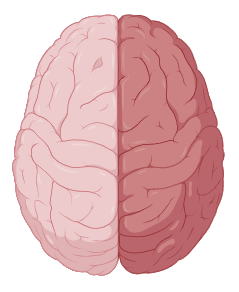
\includegraphics[scale=0.7]{Graphics/brain}
 				\end{figure}
 			\end{column}
 			
 			\begin{column}{0.3\textwidth} % Left column width
 				\centering
 				\textbf{Hemisferio Derecho}\\
 				
 			
 				
 				
 			\end{column}
 		\end{columns}
 		
 		
 	\end{frame}
 
	 %---------------------------------------------------------
 	
 	\begin{frame}
 		\frametitle{Niveles organizativos de las im\'agenes visuales} 		
 	
 	
 	\begin{columns}[c] % The "c" option specifies centered vertical alignment while the "t" option is used for top vertical alignment
 		\begin{column}{0.5\textwidth} % Right column width
 			\begin{figure}
 				\centering
 				
\includegraphics[scale=0.3]{Graphics/tree}
 			\end{figure}
 			\centering
 			\textbf{Global}\\
 			Percibir y procesar el conjunto o configuraci\'on general del est\'imulo visual.
 			
 			
 		\end{column}
 		
 		
 		\begin{column}{0.5\textwidth} % Left column width
 			\begin{figure}
 				\centering
 				
\includegraphics[scale=0.43]{Graphics/leaf_branch}
 			\end{figure}
 			\centering
 			\textbf{Local}\\
 			 Analizar y procesar los detalles específicos de un estímulo visual.		
 			
 		\end{column}
 	\end{columns}
 		
 		
 	\end{frame}
 
 	 %------------------------------------------------
 	\begin{frame}
 		\frametitle{Asimetr\'ia hemisf\'erica en la percepci\'on global/local}
 		
 		\begin{columns}[c] % The "c" option specifies centered vertical alignment while the "t" option is used for top vertical alignment
 			\begin{column}{0.3\textwidth} % Right column width
 				\centering
 			\textbf{Hemisferio Izquierdo}\\
 				$\downarrow$\\
 				\textbf{Percepci\'on Local}
 				
 				
 			\end{column}
 			
 			\begin{column}{0.3\textwidth}
 				\centering
 				\begin{figure}     				
 					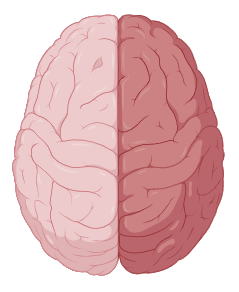
\includegraphics[scale=0.7]{Graphics/brain}
 				\end{figure}
 			\end{column}
 			
 			\begin{column}{0.3\textwidth} % Left column width
 				\centering
 				\textbf{Hemisferio Derecho}\\
 				
 				$\downarrow$\\
 				\textbf{Percepci\'on Global}
 				
 				
 			\end{column}
 		\end{columns}
 		
 		
 	\end{frame}
     
      %------------------------------------------------
    % \begin{frame}
    % 	\frametitle{Estudios sobre lateralizaci\'on hemisf\'erica}
    % 	
    % 	\begin{figure}
    % 		\centering
    % 		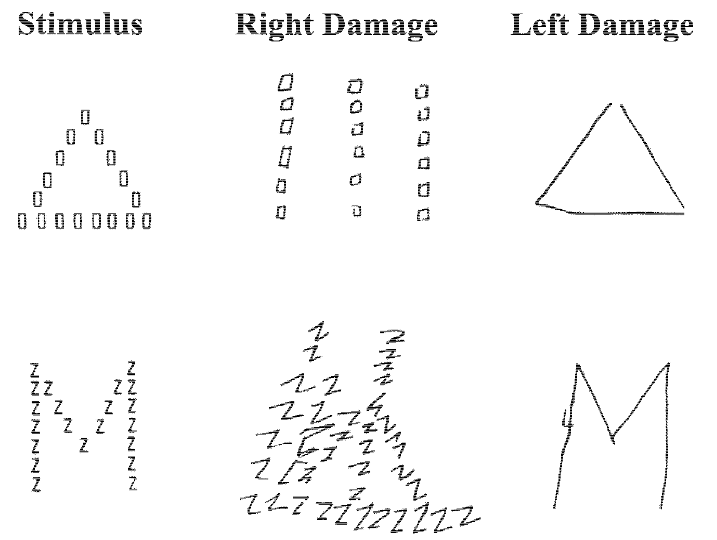
\includegraphics[scale=0.4]{Graphics/global_local}
    % 	\end{figure}
    %
    % 	
    % \end{frame}
     
    
     
     %------------------------------------------------
     \begin{frame}
     	\frametitle{Frecuencia espacial de est\'imulos visuales}
     
     	
     	Una imagen compleja puede descomponerse en componentes más simples, que varían en frecuencias diferentes.
     
    	\begin{figure}[h!]
    		\centering
    	   	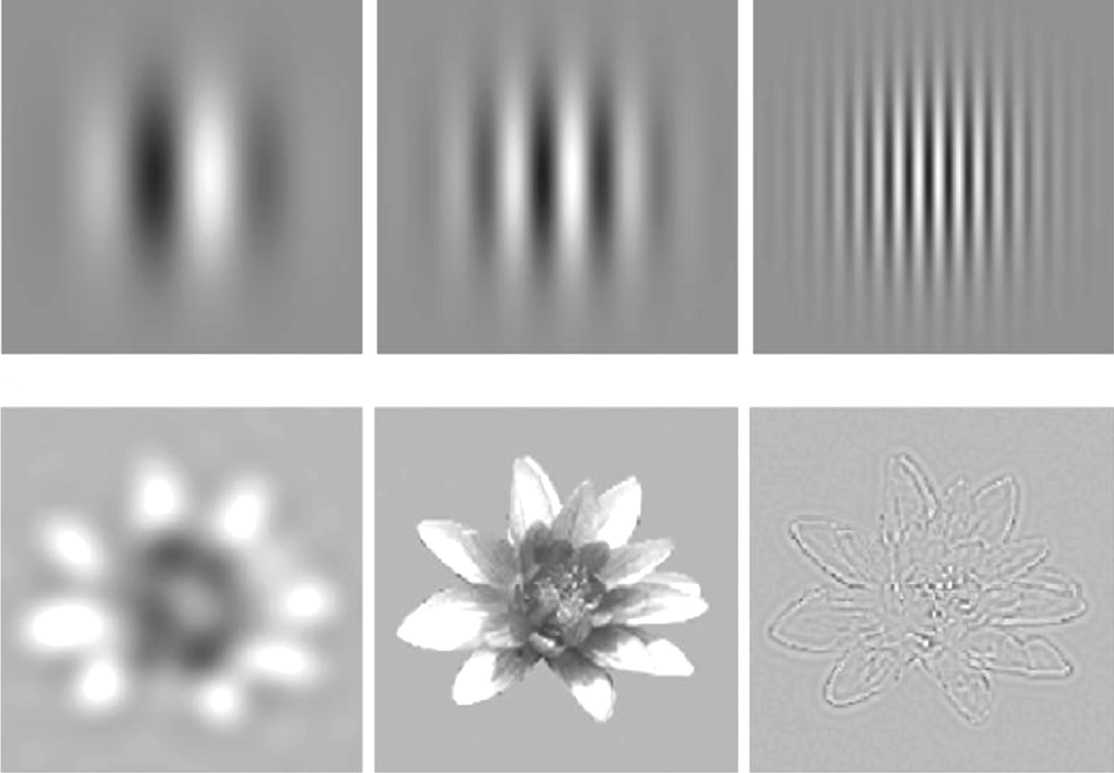
\includegraphics[scale=0.3]{Graphics/sp}
    	\end{figure} 	
     	
     	
     \end{frame}
	
	%------------------------------------------------
	\begin{frame}
		\frametitle{Teor\'ia del Doble Filtraje por Frecuencia}
		
		\begin{columns}[c] % The "c" option specifies centered vertical alignment while the "t" option is used for top vertical alignment
			\begin{column}{0.5\textwidth} % Right column width
				\begin{enumerate}
					\item Seleccionar un rango de operación en el espacio de frecuencias espaciales, de acuerdo con la escena visual a analizar.
					\item Distribuir la información a los dos hemiferios.
				\end{enumerate}	
				
			\end{column}
		
			\begin{column}{0.5\textwidth} % Left column width
			\begin{figure}[h!]
				\centering
				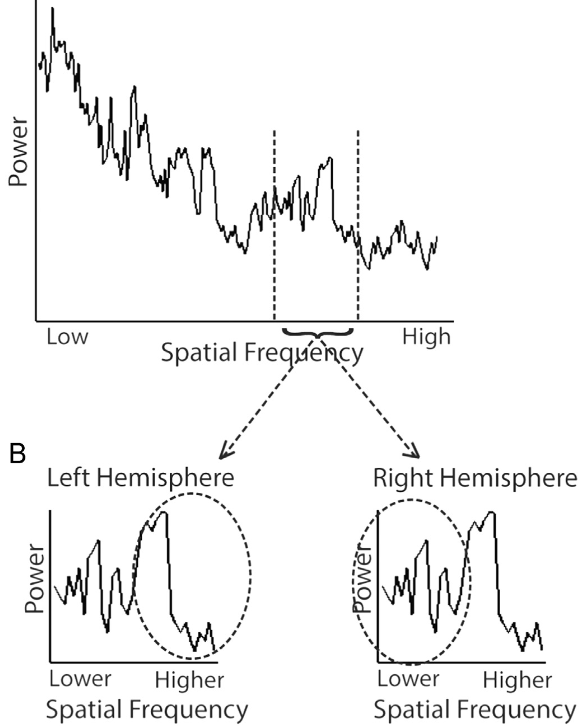
\includegraphics[scale=0.3]{Graphics/dff}
			\end{figure} 	
				
				
			\end{column}
		\end{columns}
		
		
		
		
	\end{frame}
	%------------------------------------------------
	\begin{frame}
		\frametitle{Frecuencia espacial de est\'imulos visuales}
		
		\begin{columns}[c] % The "c" option specifies centered vertical alignment while the "t" option is used for top vertical alignment
			\begin{column}{0.3\textwidth} % Right column width
				\centering
				Hemisferio Izquierdo\\
				$\downarrow$\\
				detalles finos, aspectos locales\\
				$\downarrow$\\
				frecuencias espaciales altas
				
				
			\end{column}
			
			\begin{column}{0.3\textwidth}
				\begin{figure}
					\centering
					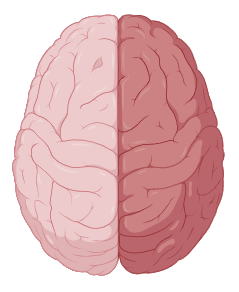
\includegraphics[scale=0.7]{Graphics/brain}
				\end{figure}
			\end{column}
			
			\begin{column}{0.3\textwidth} % Left column width
				\centering
				Hemisferio Derecho\\				
				$\downarrow$\\
				aspectos globales\\
				$\downarrow$\\
				frecuencias espaciales bajas
				
				
			\end{column}
		\end{columns}
		
	
		
		
	\end{frame}
 %-----------------------------------------------------
	\begin{frame}
		\frametitle{fMRI}
		\begin{block}{}
			La resonancia magnética funcional (fMRI) es una técnica no invasiva para estudiar
			la activación cerebral con gran resolución espacial. Mide los cambios en la oxigenación de la sangre y el flujo sanguíneo relacionados con la actividad neuronal.
		\end{block}
	

		
	\end{frame}
	
	%------------------------------------------------
	
	\begin{frame}
		\frametitle{pRF}
	
		
		
		
	\end{frame}
	
	
	%------------------------------------------------
	\begin{frame}
		\frametitle{Mapa Retinot\'opico}
		
			\begin{columns}[t] % The "c" option specifies centered vertical alignment while the "t" option is used for top vertical alignment
			\begin{column}{0.5\textwidth} % Right column width
				\centering
				\begin{equation}
					P(H|E) = \dfrac{P(E|H)P(H)}{P(E)}
				\end{equation}
				
				
			\end{column}
			\begin{column}{0.5\textwidth} % Left column width
				\centering
				\begin{itemize} 			
					\item $H$ es la deformación particular de la superficie cortical.		
					\item $E$ es un conjunto particular de mediciones retinotópicas.
				
				\end{itemize}	
				
				
			\end{column}
		\end{columns}
		

	\end{frame}


	\section{Objetivos} % Sections are added in order to Organize your presentation into discrete blocks, all sections and subsections are automatically output to the table of contents as an overview of the talk but NOT output in the presentation as separate slides

%------------------------------------------------
\begin{frame}
	\frametitle{Objetivo General}
	El objetivo general de este estudio es analizar la especializaci\'on hemisférica en el procesamiento visual del cerebro humano.
	
	
	%		
\end{frame}

\begin{frame}
	\frametitle{Objetivos Espec\'ificos}
	\begin{itemize}
		\item[1.]  Aplicar modelos que estiman la frecuencia espacial preferida de los v\'ertices corticales.
		
		\item[2.] Implementar modelos estadísticos para explicar las diferencias en las frecuencias preferidas de los v\'ertices corticales entre hemisferios.	
		
		\item[3.] Analizar la lateralización hemisférica en diferentes áreas visuales.
	\end{itemize}
	
	
	%		
\end{frame}
	
	%------------------------------------------------
	\section{Modelos}
	%------------------------------------------------
	\begin{frame}
		\frametitle{Estimaci\'on de per\'iodo preferido}
		
			\begin{columns}[t] % The "c" option specifies centered vertical alignment while the "t" option is used for top vertical alignment
			\begin{column}{0.5\textwidth} % Right column width
				\centering
				\begin{equation}
					\hat{\beta}_b(w_l) = A_b \cdot \exp\left(\frac{-(\log_2(w_l) + \log_2(p_b))^2}{2\sigma_b^2}\right)
				\end{equation}	
				
				
			\end{column}
			\begin{column}{0.5\textwidth} % Left column width
				\centering
				\begin{itemize} 			
					\item \(\hat{\beta}_b(w_l)\): Respuesta BOLD promedio en el intervalo de excentricidad \(b\) a la frecuencia espacial \(w_l\).		
					\item \(A_b\): Ganancia de respuesta.
					\item \(p_b\): Per\'iodo preferido.
					\item \(\sigma_b\): Ancho de banda medido en octavas.
				\end{itemize}	
				
				
			\end{column}
		\end{columns}
		
		
	
	\end{frame}
	%------------------------------------------------
		%------------------------------------------------
	\begin{frame}
		\frametitle{Modelos lineales mixtos}
		
		
			\begin{itemize}
				\item \textbf{Modelo Nulo:}	\\			
				\begin{equation}
					\text{Período Preferido} \sim 1 + (1 | \text{Sujeto}) + (1 | \text{Estímulo})	
					\label{m_1}
				\end{equation}
				
				\item\textbf{Modelo con Excentricidad:}\\			
				\begin{equation}
					\text{Período Preferido} \sim \text{Excentricidad} + (1 | \text{Sujeto}) + (1 | \text{Estímulo})	
					\label{m_2}
				\end{equation}
				
				\item \textbf{Modelo Aditivo con Excentricidad y Hemisferio:}\\				
				\begin{equation}
					\text{Período Preferido} \sim \text{Excentricidad} + \text{Hemisferio} + (1 | \text{Sujeto}) + (1 | \text{Estímulo})	
					\label{m_3}
				\end{equation}
			
				\item \textbf{Modelo con Interacci\'on de Excentricidad y Hemisferio:}\\				
				\begin{equation}
					\text{Período Preferido} \sim  \text{Excentricidad} \times \text{Hemisferio} + (1 | \text{Sujeto}) + (1 | \text{Estímulo})	
					\label{mlm_pp}
				\end{equation}
				
				
			\end{itemize}
		
		
	\end{frame}
	%------------------------------------------------
	\section{Resultados}
	%------------------------------------------------
	\begin{frame}
		\frametitle{Tama\~no de pRF crece con la excentricidad}
				
		\begin{figure}[h!]
			\centering
			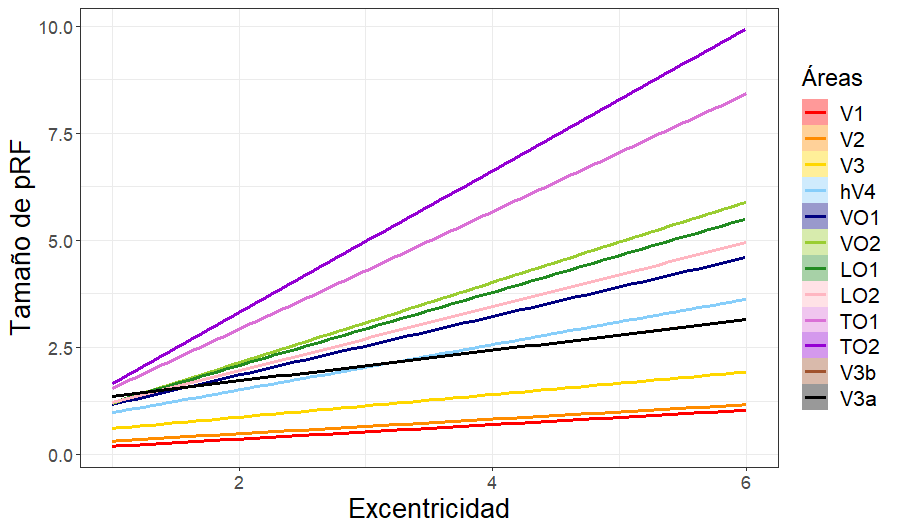
\includegraphics[scale=0.5]{../../../thesis_temp/document/Graphics/size_vs_eccen_bayesian}
		\end{figure}
		
	\end{frame}
	
	%------------------------------------------------
	\begin{frame}
		\frametitle{Per\'iodo preferido y excentricidad}
		
		\begin{figure}[h!]
			\centering
			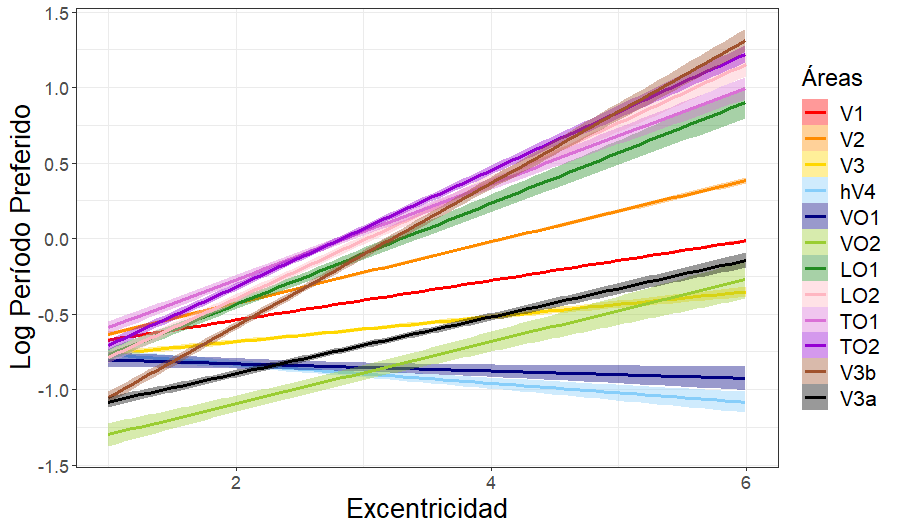
\includegraphics[scale=0.5]{../../../thesis_temp/document/Graphics/pp_vs_eccen}
		\end{figure}
		
		
		
	\end{frame}
	
	%------------------------------------------------
	%------------------------------------------------
	\begin{frame}
		\frametitle{Tabla con resultados}
		\begin{figure}
			\centering
			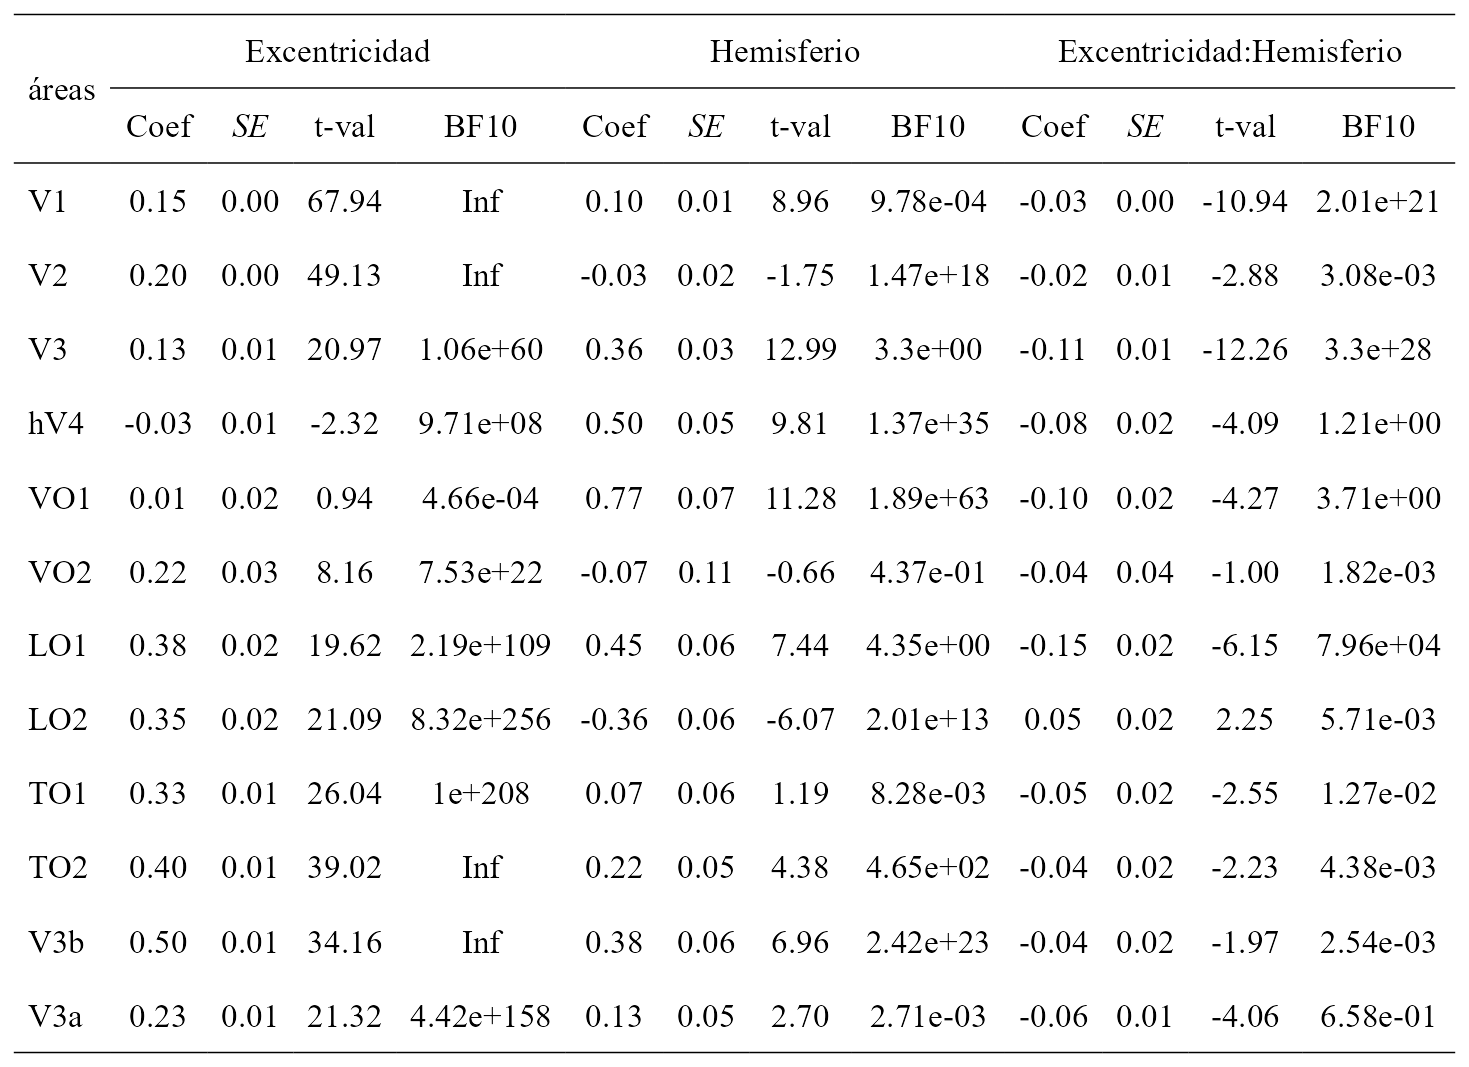
\includegraphics[scale=0.45]{Graphics/table_pp}
		\end{figure}
		
	\end{frame}
	
	%------------------------------------------------
		%------------------------------------------------

	
	%------------------------------------------------
	
	%------------------------------------------------
	%------------------------------------------------

	%------------------------------------------------
	\section{Conclusión}
	%------------------------------------------------
	
	
	\begin{frame}
		
        \centering		
		\LARGE Gracias
		
		
		
		
	\end{frame}
	

	
\end{document} 
